%\usepackage{algorithm}
%\usepackage{algorithmic}

\chapter{连通区域的预分割}
由上述章节可知,利用灰度曲面方向角模型来处理原始角毛藻显微灰度图像可以得到五张灰度特征图。其中$Map_{xz}$和$Map_{yz}$的灰度映射值较大,因此保留有大量的角毛和细胞边缘特征信息,可以更好的分割具有噪声的低对比度角毛藻显微图像的角毛。因此在这一章节中,将主要利用$Map_{xz}$和$Map_{yz}$来进行预分割的一系列操作,通过这些操作产生的结果将被用来作为支持向量机的训练样本。本章所使用的方法主要分为大津法和最大连通域的选取。
\section{大津法}
大津法(又称:最大类间方差法,OTSU)是由日本学者大津展之\cite{otsu1975threshold}于1979年提出的,是一种自适应的确定阈值来实现图像二值化的高效方法。大津法通过图像灰度特性将图像分为目标和背景两部分,通过选取目标和背景间的最大类间方差和最小类内方差来确定最佳阈值。

假设$t$为将整副图像灰度级划分为两类的阈值:$C_{0}=(0,1,...,t)$和$C_{1}=(t+1,t+2,...,L-1)$。$C_{0}$和$C_{0}$的概率分别表示为:
\begin{equation}
\omega_{0}=\sum_{i=0}^{t}P_{i}=\omega(t)
\end{equation}

\begin{equation}
\omega_{1}=\sum_{i=t+1}^{L-1}P_{i}=1-\omega(t)
\end{equation}

均值分别表示为:
\begin{equation}
\mu_{0}=\sum_{i=0}^{t}iP_{i}/\omega_{0}=\mu(t)/\omega(t)
\end{equation}

\begin{equation}
\mu_{1}=\sum_{i=t+1}^{L-1}iP_{i}/\omega_{1}=\frac{\mu_{T}(t)-\mu(t)}{1-\omega(t)}
\end{equation}

其中,$\mu(t)=\sum_{i=0}^{t}iP_{i}$,$\mu_{T}(t)=\sum_{i=0}^{L-1}iP_{i}$。对于任意的t值,都满足:$\omega_{0}\mu_{0}+\omega_{1}\mu_{1}=\mu_{T}$且$\omega_{0}+\omega_{1}=1$。

$C_{0}$和$C_{0}$的方差分别表示为:
\begin{equation}
\sigma_{0}^{2}=\sum_{i=0}^{t}(i-\mu_{0})^2P_{i}/\omega_{0}
\end{equation}

\begin{equation}
\sigma_{1}^{2}=\sum_{i=t+1}^{L-1}(i-\mu_{1})^2P_{i}/\omega_{1}
\end{equation}
定义类内方差为:
\begin{equation}
\sigma_{w}^{2}=\omega_{0}\sigma_{0}^{2}+\omega_{1}\sigma_{1}^2
\end{equation}
类间方差为:
\begin{equation}
\sigma_{B}^{2}=\omega_{0}(\mu_{0}-\mu_{T})^{2}+\omega_{1}(\mu_{1}-\mu_{T})^{2}=\omega_{0}\omega_{1}(\mu_{1}-\mu_{0})^{2}
\end{equation}
总体方差为:
\begin{equation}
\sigma_{T}^{2}=\sigma_{w}^{2}+\sigma_{B}^2
\end{equation}
引入判别准则:
\begin{equation}
\eta(t)=\frac{\sigma_{B}^{2}}{\sigma_{T}^{2}}
\end{equation}
将阈值$t$从图像最小灰度级到最大灰度级依次设置,并计算相应的值,比较所有$\eta(t)$值大小,找出$\eta(t)$取最大值时的$t^{*}值$:
\begin{equation}
t^{*}=\argmax_{0\le t\le L-1}\eta(t)
\end{equation}
目标和背景之间的类间方差越大说明目标和背景之间的灰度差别越大,与之相反,二者间的类间方差越小说明目标和背景之间的灰度差别越小即灰度分布越均匀,若出现错分现象即部分背景被错误地分为目标区域或部分目标被错误地分为背景区域都会使这两部分的差别变小,所以使错分几率达到最小就意味着需要获取最大的类间方差。


\section{实验结果}
首先采用大津法将灰度映射图$Map_{xz}$和$Map_{yz}$转化成二值图像,转化后的两幅二值图像包含两类像素即目标像素和背景像素。

然后利用MATLAB函数bwlabel标记两幅二值图像的四连通领域,被标记为0的像素为背景,其余标记如被标记为1的像素组成第一区域,被标记为2的像素组成第二区域。保留二值图像中的最大连通区域即像素值最多的区域并且移除二值图像中的其他区域,可以得到两幅保留较多角毛藻特征信息的二值图像。

因为原始角毛藻灰度图像中的噪声没有方向性和规律性,并且比较杂乱,不能同时在两幅得到的二值图像上得到高的灰度值,所以需要对两幅得到的二值图像使用逻辑“与”(AND)操作来尽量减少较为显著的噪声从而更加突出角毛藻的脚毛和细胞边缘信息。最终可以得到一个精确但是仍然缺少某些特征信息的不完整的角毛藻二值预分割结果。所得的预分割结果将会被用来作为支持向量机训练过程中的训练样本。

如图\ref{trainingsampleresult}所示为实验结果:
\begin{figure}
\centering
    \begin{minipage}[b]{0.45\linewidth}
    \centering
    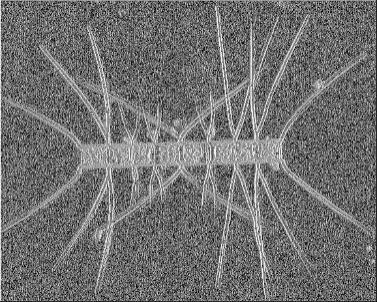
\includegraphics[width=0.9\linewidth]{mapxz.jpg}
      \centerline{(a) xz方向灰度映射图}\medskip
  \end{minipage}
  \begin{minipage}[b]{0.45\linewidth}
    \centering
    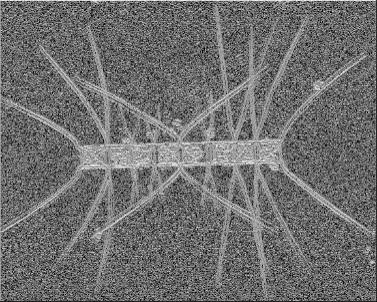
\includegraphics[width=0.9\linewidth]{mapyz.jpg}
      \centerline{(b) yz方向灰度映射图}\medskip
  \end{minipage}
   \begin{minipage}[b]{0.45\linewidth}
    \centering
    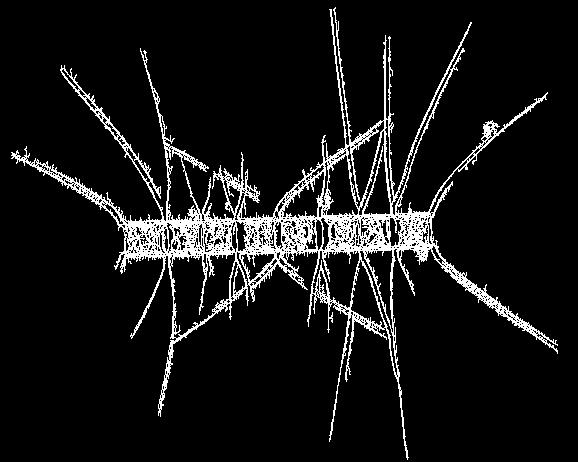
\includegraphics[width=0.9\linewidth]{xz.jpg}
      \centerline{(c) xz方向对应处理结果}\medskip
  \end{minipage}
  \begin{minipage}[b]{0.45\linewidth}
    \centering
    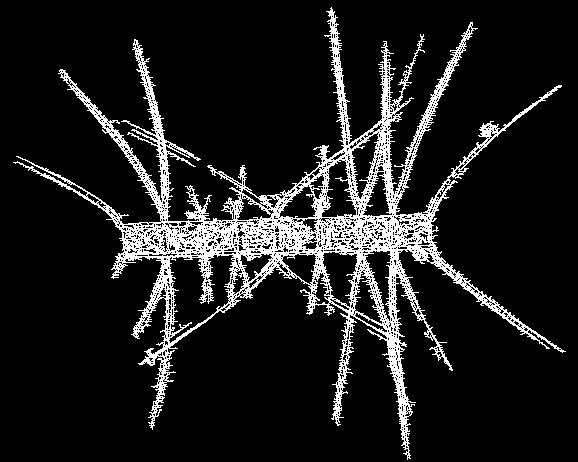
\includegraphics[width=0.9\linewidth]{yz.jpg}
      \centerline{(d) yz方向对应处理结果}\medskip
  \end{minipage}
   \begin{minipage}[b]{0.45\linewidth}
    \centering
    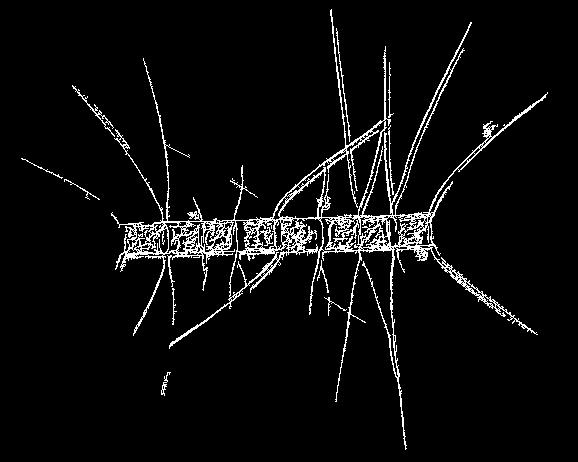
\includegraphics[width=0.9\linewidth]{traingingsample.jpg}
      \centerline{(e) 最终预分割结果}\medskip
  \end{minipage}
 \caption{大津法二值化与选取最大连通区域的预分割结果}
  \label{trainingsampleresult}
\end{figure}

\section{本章小结}
本章主要使用大津法和选取最大连通域来获取角毛藻显微图像的预分割结果。首先选择xz和yz方向的灰度映射图进行大津法二值化,然后使用最大连通域填充,最后通过逻辑“与”操作获取最终的预分割结果,得到的预分割结果将作为后续支持向量机分类训练过程的训练样本。
